\chapter{预后模型的设计与实现}
\label{cha:models}

\section{模型需求与衡量标准分析}

按照实际需求,预后模型的主要目的是将不同类型的预后群体区分。与其他领域使用模型准确率进行模型的评估不同,由于医学模型的建立初衷是评估患者的实际表征的区别。按照常用模型的分类标准\cite{cancers12102802},现在学术界经常使用的是将生存数据之外的变量作为参数输入,并使用预测3年或5年生存结果或概率估计作为输出,这是一个基于时间-事件的回归问题。这种方法得到的决策树模型能够按照决策树结构中的先后顺序来判断特征重要性,而且模型能够按照节点导出一张树形图。虽然这个方法能够得到一些关于重要性的内容和一张树形图,但是考虑到这样的结果可解释性较差,所以本文在这里引入了一个新的方法。聚合层次聚类方法常常被用来将患者的临床表现分组,按照患者的临床表征相似度来区分患者的不同风险层级,从而能够让聚类方法中的区分效果更好。这里为了维持患者的分类效果,让层级效果更高,所以有必要对于患者的表征分类数量进行一定的评估,但是考虑到临床要求,分类数如果过少或者过多依然不能很好地区分患者,因为如果层次过少无法很好地细分患者的风险,如果过多则对于日常使用有一定影响,同时聚类效果也会较差,所以这里需要按照实际临床需求和实际效果进行权衡。如果能够对于患者进行分群,临床上能够对于患者的不同特征还得更好的数据,从而能够更好地评估每个患者的类型,如果将来的临床治疗方法发展,也能更好地对这些患者的实际情况进行区分,因此也能让这些患者群体的患者使用不同的治疗方法,对症治疗后的评估也能让之后的数据与之前的数据形成对比,发现不同患者群的预后效果变化,这类数据分析也能帮助患者更好地获得符合自己的治疗效果,同时也能让患者对自己的病情特征有更好的了解。然而,虽然无监督方法是探寻患者表型的有效工具,与有监督模型相比,无监督模型在对新数据的应用上有局限。这具体表现在:患者的无监督模型在对于一个数据集训练后如果得到了表型,那么这个模型虽然能够区分出多个表型,但是对于每个表型需要人工进行挑选,一般会呈现为低中高等多个等级,而这些表征等级的不同特征往往是比较独一无二的。如果要对新的数据重新进行训练,那么原先的表型很有可能会与新的表型有一些不同,对于K-means聚类,这就体现在每个簇的质心就算在新的数据上表现类似,但是依然不会完全一致,这造成了聚类方法在新的训练后依然需要人工区分新的表型。那么能否完全使用有监督模型替代呢?答案是否定的,有监督模型无法直接仅凭自身方法总结出这些特征。综上所述,结合无监督与有监督ML方法是一个可能的解决方法\cite{life12060776}。

考虑到上述需求,能否区分患者的实际表现差异更为重要,所以预后模型的价值一般使用CI进行验证,好的预后模型CI值较高。CI即为C-Index,是用来评估模型预测能力的指标,它主要计算了模型预测值与真实之间的区分度。在肿瘤患者的实际预后精确的衡量中,我们很多时候是从两个层面进行评估,其中一个是使用拟合优度检验指标进行衡量,这个标准主要用于衡量分类结果中的各个分类的频数的期望,从总体分布状况上。不过在医学临床应用角度中,一个更重要的指标是对模型精度的衡量,即使用C-index来衡量预测结果的准确性。相比于使用常见模型使用的均方差等,更常用的便是使用上文提及的C-Index进行衡量,计算结果发生概率和实际概率的一致性是我们主要的目的。C-index的作用便是预测预期结果和实际输出相一致的概率,在二分类问题中,正类结果大于负类结果即可累计从而计算概率。C-index通常先对数据进行预处理,将使用的验证数据集中的实例两两分为许多对子,这些对子中不是两两配对即可,而是要生成所有的对子组合,所以如果验证数据集中一共有n条样本,那么最后生成的对子数即为$C_{n}^{2}$对。将这些对子中存在没有到达观察终点的无效样本的对子排除后,剩余的即为有效对子。在对子中,如果预测结果都与预期结果相一致,那么这些对子被称为一致对子,统计对子的数量。根据上述过程,设样本数为$n$,无效对子数为$N$,有效对子数为$A$,可以得到以下公式:

$$
CI = \frac{A}{C_{n}^{2} - N}
$$

考虑到sklearn中的相应指标是ACC,它的计算方法为:

$$
ACC = \frac{TP+TN}{TP+PN+FP+FN}
$$

而没有直接对于CI的实现,所以这里笔者使用了ROC曲线下面积AUC进行等效替换二分类模型中的CI,这是因为在二分类模型中AUC和CI是相同的,而多分类模型中的则调用其他sklearn之外的专用库函数实现。

\section{使用分类模型建模}

\subsection{决策树}

决策树使用树形结构来进行分类,通常决策树一般在分类患者的具体病情中使用,而考虑到本研究指针对子宫肉瘤的患者,而如果用来分类原发部位则不太符合临床标准,因为患者的具体的原发部位使用核磁共振或超声图像进行诊断会更加精确而直接,同时考虑到对患者进行诊断本身就是医生的工作,如果用模型进行分类不但会与医院本身的工作流程重复,数据内容也不支持建模,同时模型的准确率也很少会高于人工诊断结果,所以不需要使用决策树来对原发部位等信息进行分类。所以这里则直接用决策树来进行患者三年生存概率的二分类模型建立。

决策树选择好特征后,根节点开始是的非叶子节点分别是决策树的树中的特征范围,而决策树中的叶子节点则表示了最终的分类结果。决策树使用了基尼系数来衡量特征空间的有序性,决策树通过改变数据划分来使得信息增益最大,即使得最终的基尼系数最大。基尼系数。

\subsubsection{决策树中的特征重要性分析}

这里使用的输入数据中,其他输入变量如章\ref{cha:analyse}中分析得到,分别为年龄、种族、原发部位、肿瘤大小、分期、化疗情况、分级,考虑到年龄为区间分类变量,所以需要对其进行编码化,按照顺序分别将其编码为0,1,2,3,4...等,而训练的分类目标则是三年死亡率。经过训练后,可以得到如下表\ref{tab:dt_importance}的特征重要性表:

\begin{table}[htb]
    \centering
    \begin{minipage}[t]{0.8\linewidth} 
    \caption[决策树得到的特征重要性]{决策树得到的特征重要性}
    \label{tab:dt_importance}
      \begin{tabularx}{\linewidth}{XXXXXXX}
        \toprule[1.5pt]
        {\heiti Age} & {\heiti Race} & {\heiti PS} & {\heiti TS} & {\heiti Stage} & {\heiti Chemo} & {\heiti Grade} \\\midrule[1pt]
        0.0210 &  0.0028 & 0.0035 & 0.0037 & 0.0295 & 0.0031 & 0.053 \\
        high & low & low & low & high & low & high \\
        \bottomrule[1.5pt]
      \end{tabularx}
    \end{minipage}
  \end{table}
  
根据上表可以分析得出,年龄、分期、分级相对于其他因素重要性较高,而种族、原发部位、肿瘤大小、是否化疗则相对较低。这些原因可以得到一定解释。

患者的年龄显然是一个与生存率相关的因素,年龄较大的患者免疫系统较为低下,他们的身体机能也往往较弱、呈现退行状态,而因此患者自身对于癌细胞的抵御作用较低,患者同时也有一些并发疾病,比如心血管疾病等,这些疾病让患者更有可能在治疗过程中分身乏术,很多时候死亡原因也包括因为癌症的并发症而死亡,这些因素导致患者的年龄对于死亡率有很高的影响。同时年龄较高的患者也同时是癌症的高发群体,他们更易因为致癌因素的积累等原因患癌症,同时他们也更有可能将癌症误认为老年化后自然而然得到的疾病,在数据中,可以分析得到中老年子宫肉瘤患者分期和进展程度往往明显高于青年患者,这也解释了为何老年患者的生存率明显低于青年患者。

而分期则是癌症进展的一个重要指标,如果癌症的扩散程度较高,那么患者的治疗便需要更为激进,使用一些对于患者身体有大量伤害的疗法,比如化疗和放疗等等。同时,如果患者的分期中,肿瘤细胞扩散到了周边组织,特别是淋巴细胞的侵扰,会让手术和化疗手段更难清除肿瘤细胞,而癌症细胞的扩散也就意味着复发的可能性更高,所以患者的死亡率也更高。

对于分级而言,它衡量了肿瘤细胞和它的来源组织的结构学相似度,肿瘤的细胞如果相似度高,那么它的分化程度也较高,这说明了癌症细胞由于突变导致的碱基对缺失等的变化较小,这类细胞在微观层面上和周边的原发细胞的差异较小,分化程度高。而因为高分化的细胞往往因为其组成的组织学结构较为稳定,往往嵌合为较为有序的结构,这也表明其继续分裂生长的可能性较低,速度较慢。而如果分化程度较低,甚至为未分化细胞,那么肿瘤细胞的形态上往往是无序而呈现为离散结构。一般而言,越是未分化的细胞往往更容易以较快的速度增值,这些细胞的组织学特征也让它们往往呈现为较小而不定形状态,所以也容易通过血液或组织液等途径向外扩散,所以分化较低的恶性肿瘤细胞往往意味着肿瘤本身是恶性的,对人体的威胁也较大,分级较高的患者如果没有通过及时检查,其恶性肿瘤的扩散速度相对于良性肿瘤一般会更快,这也体现了分级与分期的相关性。

虽然分期分级有一定关联,然而其却不能完全相互替代,这是因为同样分级的患者,按照发现的时间和病情进展情况会有不同的分期作为体现,这是因为分级较高的恶性肿瘤如果发现及时未扩散,那么相比于恶性程度较低但是扩散的肿瘤会更好处理,所以两者之间不会体现替代关系。同时,如果相同分期的患者之间的分级有区别,那么分级较高的患者之后的扩散会更难抑制,同时药物对于不同分级的细胞的作用也会有一定区别。分期分级作为两个衡量指标,一个体现了癌症的进展状况,一个体现了癌症的微观恶性程度。前者是癌症对于患者的宏观影响,后者体现了癌症的特性同时,也表现了癌症的之后的进展速率。所以两者相辅相成不可分割。

分析了上述影响因素较大的特征,接下来是影响较低的特征,分别是种族、原发部位、肿瘤大小、是否化疗。

其中种族影响因数较小的原因显而易见,首先数据集中采用的是美国SEER数据库的数据,其中数据来源近似,医疗水平也较为平均,而同一国家的生活方式,环境区别整体水平也差异不大,趋于同质化。如果数据来源于不同国家,可以预见的的由于不用医疗水平的差异,来自不同国家的不同人种的数据由于环境、生活方式、治疗能力的差别可能会有较大的差异。同时这个特征也体现了不同种族的人在对于子宫肉瘤的死亡率虽然存在差异,但是相比于上述的重要因素并不是主体影响因素。

原发部位体现了患者的肿瘤从哪里的组织开始生长,对于分化较高的肿瘤,肿瘤细胞本身的结构和性状会更接近原先组织,所以原先组织的生命周期特点会对肿瘤之后发展的情况有一定影响,比如卵巢原发的肿瘤相比输卵管肿瘤在相近的分化情况下可能生长速度会更快。同时,原本组织的形态特征和功能特征也会对患者的身体情况有一定影响,性腺的激素相关细胞较多,所以如果肿瘤细胞继承了原先正常细胞的激素分泌功能,患者的激素水平很可能也会受到相应的影响,而输卵管的病变如果长期影响到了输卵管的正常功能,也可能会导致卵巢等组织的功能受到影响,可能会导致患者需要切除正常组织,这也会对患者的预后结果产生较大的影响。而这个影响因素体现为较低水平的原因可能是这些影响在经过手术和相应治疗手段后比较容易去除,同时医学界也有相应的成体系的治疗方法应对,所以对于患者的预后影响较小。

考虑到子宫肉瘤对周边组织的侵扰性较强,且肿瘤切除后对于患者的影响相比于一些其他部位的肿瘤,比如脑瘤等风险更小。这是因为患者腹腔中的空间较大,较大的肿瘤对于患者的压迫作用较小,手术切除的风险相对而言也不是特别高。同时,子宫肉瘤往往会因为其侵扰性出现多个肿瘤,而肿瘤大小只能反映其中最大的一个肿瘤大小,其他肿瘤并不在考虑范围之内。较大的肿瘤在临床上有多种方法,包括分段切除、淋巴结清扫等,这些方法可以有效降低肿瘤的转移和复发概率。\cite{cabrera2021survival}所以肿瘤的大小虽然也是一个重要的特征指标,但是重要性次之。

而是否化疗对于肿瘤的影响较小是因为化疗与否是治疗手段的一部分,一般只有肿瘤进展较高的患者需要进行化疗进行术后辅助治疗。而SEER数据中,化疗数据由于患者隐私问题,所以不化疗和不知道是否化疗的数据被归为一类,这也导致了化疗对于患者的影响因数可能被削减了。

\subsubsection{决策树树形结构一览}

考虑到实际树形结构过大,难以在页面中完整显示,所以图\ref{fig:dt_tree_sturcture}仅仅列出了一部分树形结构:

\begin{figure}[!htbp]
    \centering
    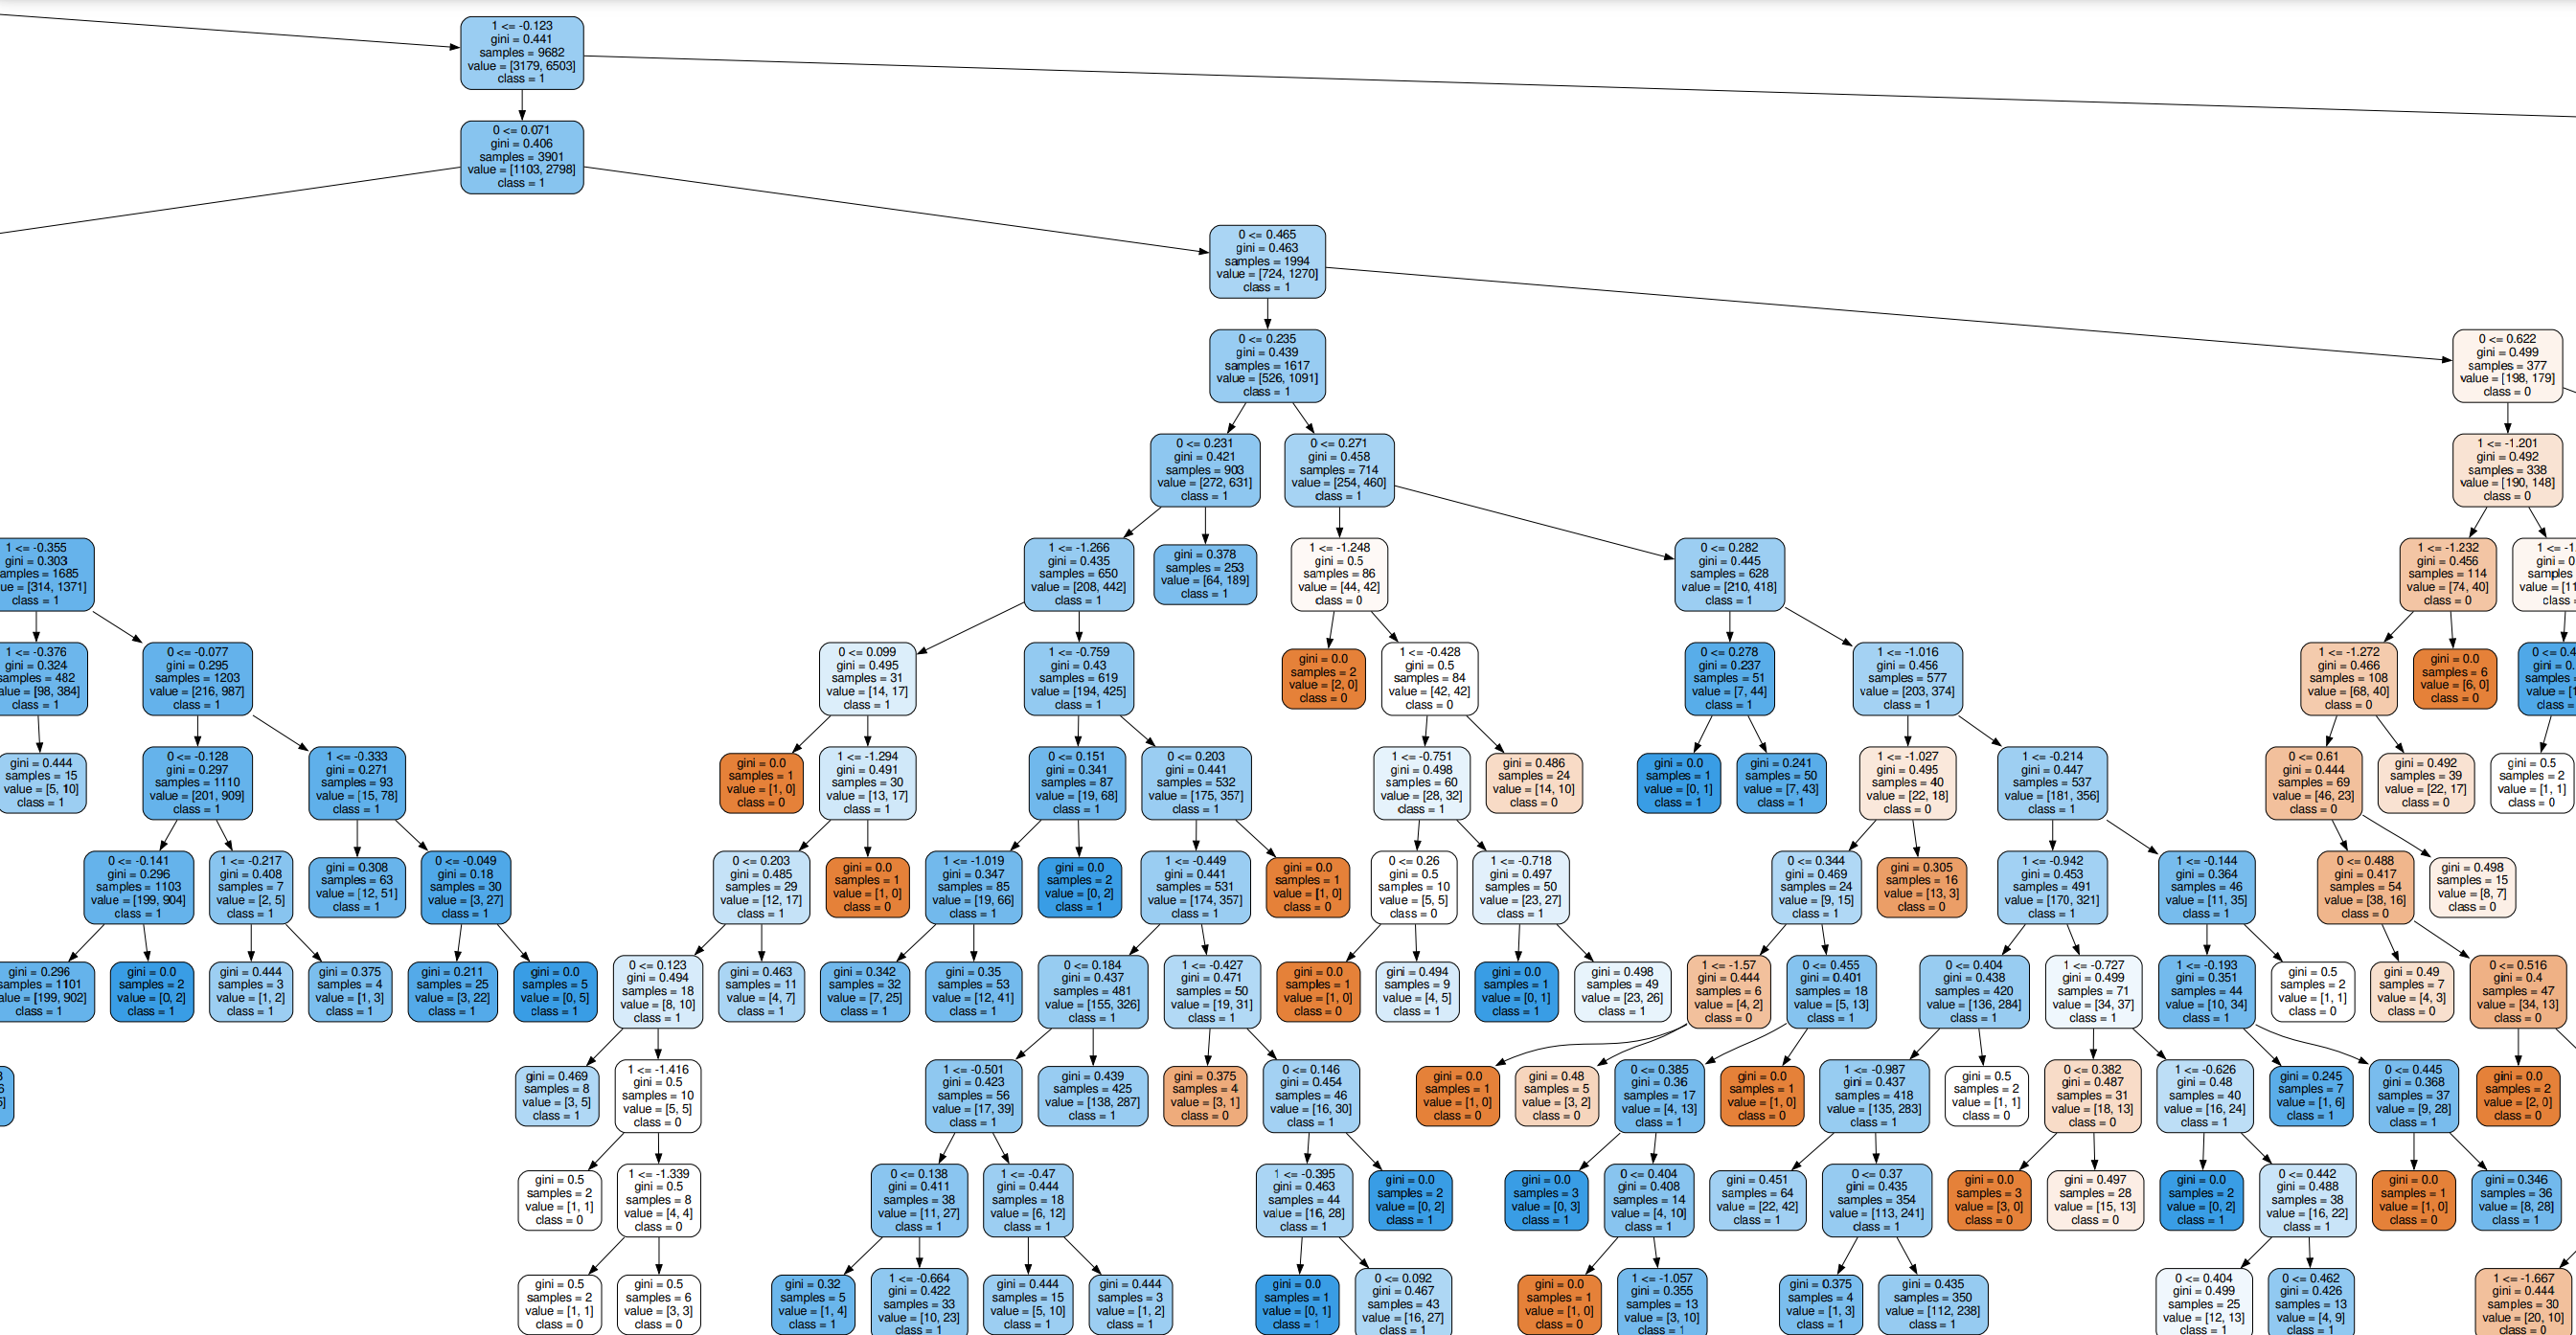
\includegraphics[scale=0.2]{dt_tree_sturcture.png}
    \caption{决策树部分结构一览} \label{fig:dt_tree_sturcture}
\end{figure}

由于特征过多,决策树使用了PCA降维来进行主成分分析,通过降维变量来提取数据的主成分向量来对数据空间进行优化。可以看到图中树的深度为15层,基尼系数从0.449开始逐层下降,最终的分类结果则在叶子节点中体现。

\subsection{随机森林}

随机森林是一种基于决策树实现的集成学习ML算法,它通过建立多个具有不同树核特征的随机决策树构建,树核特征是指这些树具有不同的深度和节点分布。按照数据中的样本权重,各个决策树不断优化其树结构和表现,最后随机森林选取其中效果最好的一类决策树,并利用它作为最终的分类模型。随机森林的生成过程相比于决策树有一定的随机性,同时训练集中的重复数据构成的不用样本权重分布也会让随机森林更好地把握数据之间的关联。由于使用随机方法构建多棵决策树,在数据量有限的训练数据中,相比于决策树,随机森林有更好的泛化效果和鲁棒性,同时它也能更好地分块处理大量数据,因为大量数据中的重复样本分布能让随机森林更好地发现数据的重要程度的不同,拟合效果和训练速度也更好和更快。

\subsection{Cox比例风险模型}

Cox比例风险模型经过章\ref{cha:analyse}的分析已经验证了它的使用前提假设在当前数据中是满足的。该模型主要基于使用风险函数表示:

$$
h(t)=h_{0}(t) \cdot exp(b_{1} \cdot 1+b_{2} \cdot 2+...+b_{p} \cdot p)
$$

风险函数表示患者在时间$t$发生死亡事件的风险。

\subsection{模型效果评估}

经过上述三个模型的训练,表\ref{tab:models_result}表示了三个模型的训练效果:

\begin{table}[htb]
    \centering
    \begin{minipage}[t]{0.8\linewidth} 
    \caption[决策树得到的特征重要性]{决策树得到的特征重要性}
    \label{tab:models_result}
      \begin{tabularx}{\linewidth}{lXX}
        \toprule[1.5pt]
        {\heiti 模型} & {\heiti 训练集C-Index} & {\heiti 测试集C-Index} \\\midrule[1pt]
        决策树 & 0.75 & 0.76 \\
        随机森林 & 0.79 & 0.78 \\
        Cox比例风险模型 & 0.80 & 0.79 \\
        \bottomrule[1.5pt]
      \end{tabularx}
    \end{minipage}
  \end{table}

从图中可以得到一些信息,决策树的拟合能力稍弱于随机森林,而由于数据量较大,所以两者在测试集中的表现差异不大,而Cox比例风险模型由于使用了风险函数进行评估,而且结果输出的是指定时间而非对于患者的特定时间的死亡风险进行评估,所以相对于对于三年死亡训练得到的二分类模型有更强的表现力,不是单单的二元分类也让它的CI指数大于二分类的前两者,这是由于一些处于边界情况的患者较难进行分类的缘故。

\section{使用聚类与分类模型结合建模}

\subsection{聚类}

\subsubsection{聚类方法与聚类数量确定}

这里分别使用K-means和层次聚类方法对数据进行聚类,轮廓系数如表\ref{tab:silhouette_coefficient}所示:

\begin{table}[htb]
    \centering
    \begin{minipage}[t]{0.8\linewidth} 
    \caption[不同聚类方法的轮廓系数]{不同聚类方法的轮廓系数}
    \label{tab:silhouette_coefficient}
      \begin{tabularx}{\linewidth}{lXXX}
        \toprule[1.5pt]
        {\heiti 方法} & {\heiti 2 clusters} & {\heiti 3 clusters} & {\heiti 4 clusters} \\\midrule[1pt]
        K-means聚类 & 0.356 & 0.239 & 0.247 \\
        层次聚类 & 0.378 & 0.337 & 0.273 \\
        \bottomrule[1.5pt]
      \end{tabularx}
    \end{minipage}
  \end{table}

其中轮廓系数是用来衡量聚类后的簇间轮廓清晰与否的指标,如果一个采样点和其所在的簇内的其他元素较为贴合,且与簇外的元素紧密程度较低,那么则可以说该次聚类的效果较好。从上图可以看到,层次聚类在当前数据集中的聚类效果好于K-means聚类,而且轮廓系数上聚类的目标类数越多,轮廓系数越低。这是因为患者的特征各有不用,在样本空间上较为弥散导致的。虽然分两类可以得到较好的聚类效果,然而两类的临床作用却较低,所以权衡后,本文使用了三类中效果表现最好的层次聚类。

\subsubsection{聚类效果评估}
  
下面的图\ref{fig:2clusters_km}和图\ref{fig:3clusters_km}是使用Kaplan-Meier曲线对聚类方法进行的效果检验:

\begin{figure}[!htbp]
    \centering
    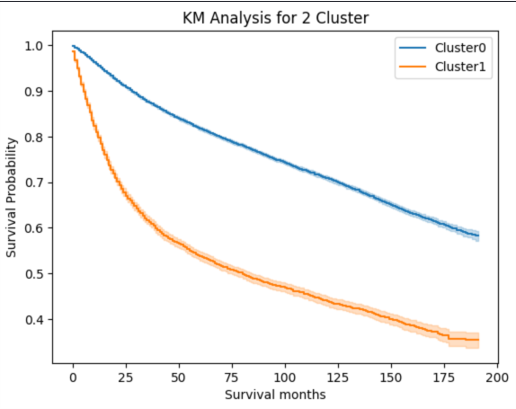
\includegraphics[scale=0.8]{2clusters.png}
    \caption{层次聚类分为两类时的Kaplan-Meier曲线} \label{fig:2clusters_km}
\end{figure}

\begin{figure}[!htbp]
    \centering
    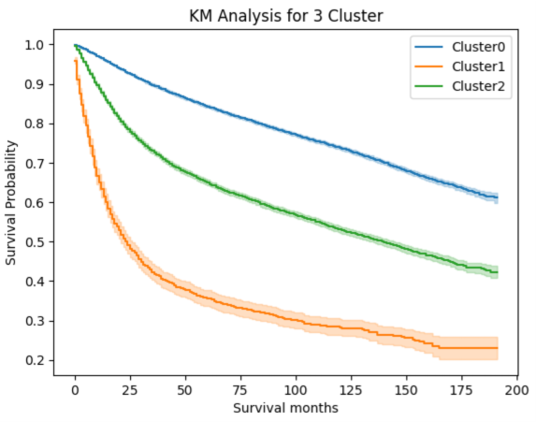
\includegraphics[scale=0.8]{3clusters.png}
    \caption{层次聚类分为三类时的Kaplan-Meier曲线} \label{fig:3clusters_km}
\end{figure}

可以看到图\ref{fig:3clusters_km}中的三类的生存率曲线存在明显的差异,这表明了就算没有将患者的生存情况纳入作为因素,仅仅凭借聚类方法生成的患者表征群仍然具有一定的生存率差异,而这差异则可明显地将患者分为三个风险等级。

在图\ref{fig:3clusters_violin}中,我们可以看到在三个患者表征群中,对于连续变量肿瘤大小而言,三个簇间区分度较好,而对于分类变量而言,三个分类则都具有不同的各个分类值的比例,区别是三者的比例分布有差异,这可能是考虑到了综合不同因素的原因。

\begin{figure}[!htbp]
    \centering
    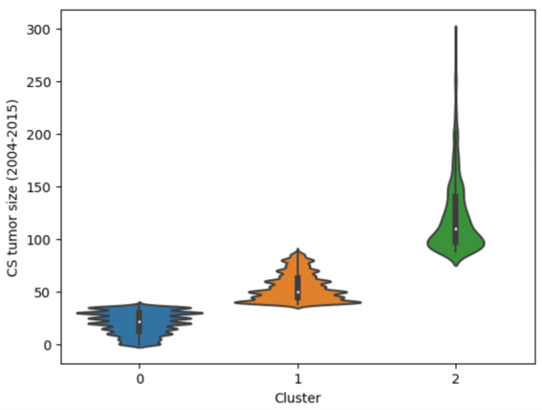
\includegraphics[scale=0.8]{3clusters_violin.png}
    \caption{层次聚类分为三类时的肿瘤大小变量小提琴图} \label{fig:3clusters_violin}
\end{figure}

总体而言,层次聚类方法能够将患者分为三个生存率有明显差异而不交叉的簇,而对于其中的连续变量也有较好的划分性能,具有一定的参考使用价值。

\subsubsection{模型效果评估}

在将聚类标签作为分类目标,在训练集和测试集中分别标记,并使用随机森林模型训练后,该模型的训练集CI为0.97,测试集CI为0.95。可以清晰的得到这个模型具有很好的分类效果,原因是分类的目标本身就是聚类得到的空间点位相近的簇,分类模型对于这种比较清晰明确的区间分类拟合效果很好。

\section{预后模型总结}

本章主要介绍了两类分类模型的实现,其一是基于预测患者的三年死亡与否和死亡时间的分类模型,在这类模型中,本文直接使用监督学习方法进行预测,决策树和随机森林的结果比较相近,两者接近于使用Cox比例风险模型进行分类的结果。而第二类则是使用聚类方法配合监督学习进行的患者表征分类,这类方法不直接得到患者的具体死亡情况,而是根据患者的病理特征对患者群体进行分类,得到多个死亡风险有差异的表征群(簇),这种方法具有较好的临床参考价值和极高的一致性参数(CI),但是考虑到这种方法的目标并非直接得到死亡率,而不同群体之间也不存在百分百的确定生存或死亡,其实际的准确率达不到结果的0.95,但是考虑到实际患者的生存率取决于多方面影响,并没有与病理得到的参数强相关,进行死亡率分类的模型最后的CI性能往往被限制在0.8左右,所以这种方法为如何相关研究提供了一项新的思路,具有一定的参考价值。